\chapter{Entreprise}
\label{Entreprise}
\thispagestyle{fancy}

\section{Histoire}
\label{Entreprise: histoire}
Aldebaran (anciennement Aldebaran Robotics) est une société Française de robotique humanoïde, fondée en 2005 par Bruno Maisonnier. 

\subsection{Le premier robot, Nao}
\label{Entreprise:Histoire:Nao}
Constituée au départ d'une équipe de douze collaborateurs, la toute jeune entreprise se fixe comme objectif de développer des robots humanoïdes et de les commercialiser au grand public, en tant que "nouvelle espèce bienveillante à l'égard des humains". Après trois années de recherche et développement, la société dévoile en 2008 son tout premier produit: Nao. La participation du robot humanoïde à divers évènements internationaux, comme par exemple la RoboCup ou encore l'Exposition Universelle de Shanghai en 2010 participe à sa popularisation auprès des laboratoires de recherche, des universités et des développeurs. Une seconde génération de robot Nao apparait en 2011 (dit Nao Next Gen). L'entreprise dévoile durant la même période un nouveau projet, en partenariat avec différents acteurs de la recherche, visant à créer un véritable robot d'assistance à la personne, Roméo. 

\subsection{La famille s'agrandit}
\label{Entreprise: La famille Aldebaran}
Lors de l'année 2012, Aldebaran Robotics est racheté par SoftBank, société spécialisée dans le commerce électronique au Japon, et devient alors Aldebaran. Débute alors la conception d'un tout nouveau produit, le robot humanoïde Pepper. Dévoilé au grand public en 2014, il est dans un premier temps vendu au Japon auprès des entreprises. Les premiers clients à en bénéficier seront les magasins de téléphonie mobile du groupe SoftBank. Les ventes s'ouvrent dans un second temps aux particuliers Japonais. La société compte aujourd'hui plus de 400 collaborateurs et poursuit le développement de ses trois produits afin de les améliorer et de conquérir de nouveaux marchés (en Europe , en Chine et aux États-Unis).

\section{Les produits}
\label{Entreprise: Les produits}
Aldebaran commercialise à ce jours deux produits: Nao et Pepper. Le robot Roméo est une plateforme de recherche. 

\subsection{Nao}
\label{Entreprise: Les produits: Nao}
Nao est un robot humanoïde de 58 cm de hauteur. Son public cible est principalement les laboratoires de recherche et le monde de l'éducation (allant des écoles primaires aux universités). Il est actuellement le produit le plus connu de l'entreprise auprès du grand public. 

\begin{figure}[h]
	\centering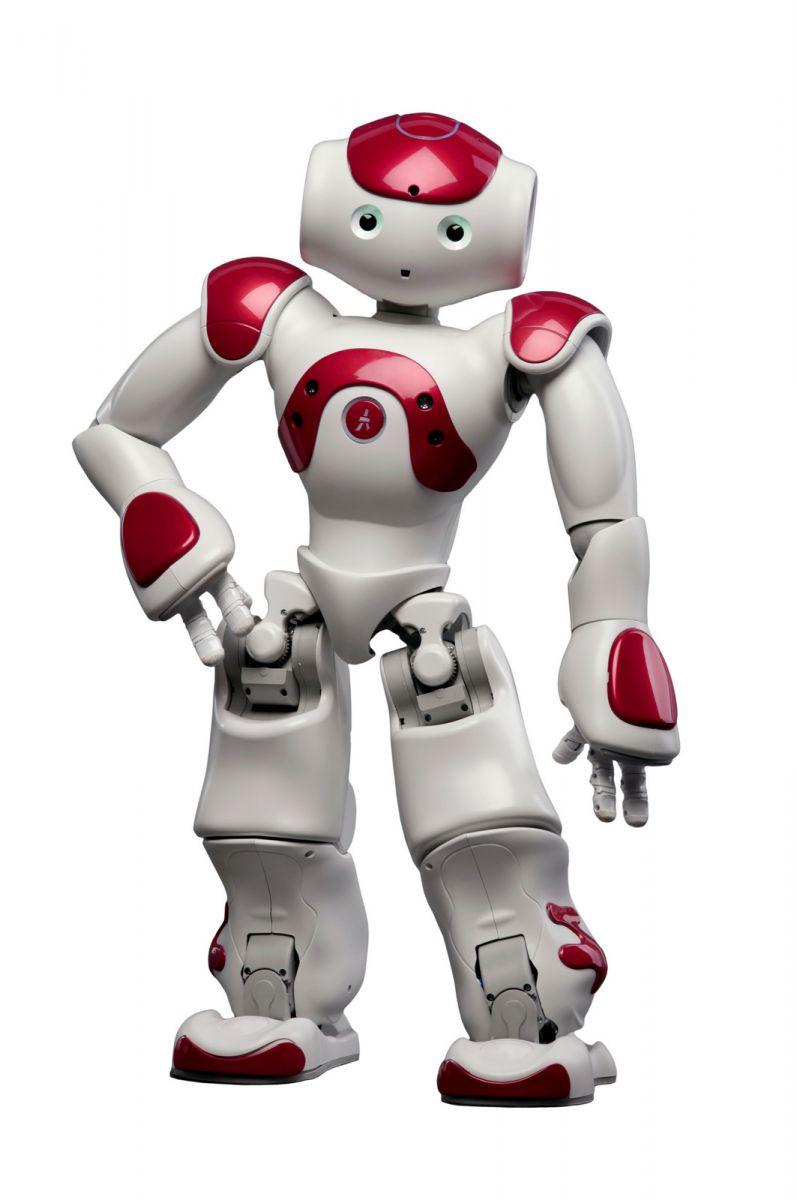
\includegraphics[height=7cm]{images/nao.jpg}
	\caption{Le robot humanoïde Nao.}
	\label{fig:Robot humanoïde Nao}
\end{figure}

\paragraph{Caractéristiques techniques}
\label{Entreprise:Les produits: Nao: Caractéristiques techniques}
Caractéristiques techniques de la dernière version de Nao (V5, Evolution). \ref{tab: Caractéristiques technique de Nao}

\begin{table}[h]
\begin{tabular}{ | l | p{8cm} | }
\hline
\multicolumn{2}{|c|}{Caractéristiques générales} \\
\hline
Dimensions & 574 x 311 x 275 mm \\
\hline 
masse & 5,4 kg \\
\hline 
Degrés de liberté  & 25 \\
\hline
Processeur & Intel Atom Z530 \newline 1.6 GHz \newline RAM: 1GB \newline Mémoire flash: 2GB  \newline Micro SDHC: 8 GB \\
\hline
Système d'exploitation & Middleware Aldebaran NAOqi basé sur un noyau Linux \\
\hline
Connectivité & Wi-Fi, Ethernet, USB \\
\hline
Batterie & Autonomie: 90 minutes en usage normal \newline Energie: 48.6 Wh \\
\hline 
Vision & Deux caméras frontales 2D, 1220p, 30ips \\
\hline
Audio & Sortie: 2 haut-parleurs stéréo \newline 4 microphones directionnels \newline moteur de reconnaissance vocale Nuance  \\
\hline
Capteurs & 2 capteurs infra-rouges, résistance sensible à la pression, centrale inertielle, 2 systèmes sonars, 3 surfaces tactiles \\
\hline
\end{tabular}
\caption[Caractéristiques technique de Nao]{Caractéristiques techniques de la dernière version commerciale  de Nao}
\label {tab: Caractéristiques technique de Nao}
\cite{NaoTech}
\end{table}

\subsection{Pepper}
\label{Entreprise: Les produits: Pepper}
Dernier né d'Aldebaran, le robot Pepper est conçu pour vivre au côté des humains. Imaginé au départ pour accompagner et informer les clients dans les magasins de téléphonie du groupe japonais SoftBank, l'entreprise cherche à présent à placer son produit chez les particuliers. Le robot se base sur la structure software et hardware de Nao. Cependant, contrairement à son compagnon Nao, celui-ci se déplace non pas grâce à une paire de jambes, mais via trois roues omnidirectionnelles, facilitant son déplacement. A noter également que Pepper est équipé d'une tablette tactile sur son torse afin de faciliter les interactions Homme-Machine.

\begin{figure}[h]
	\centering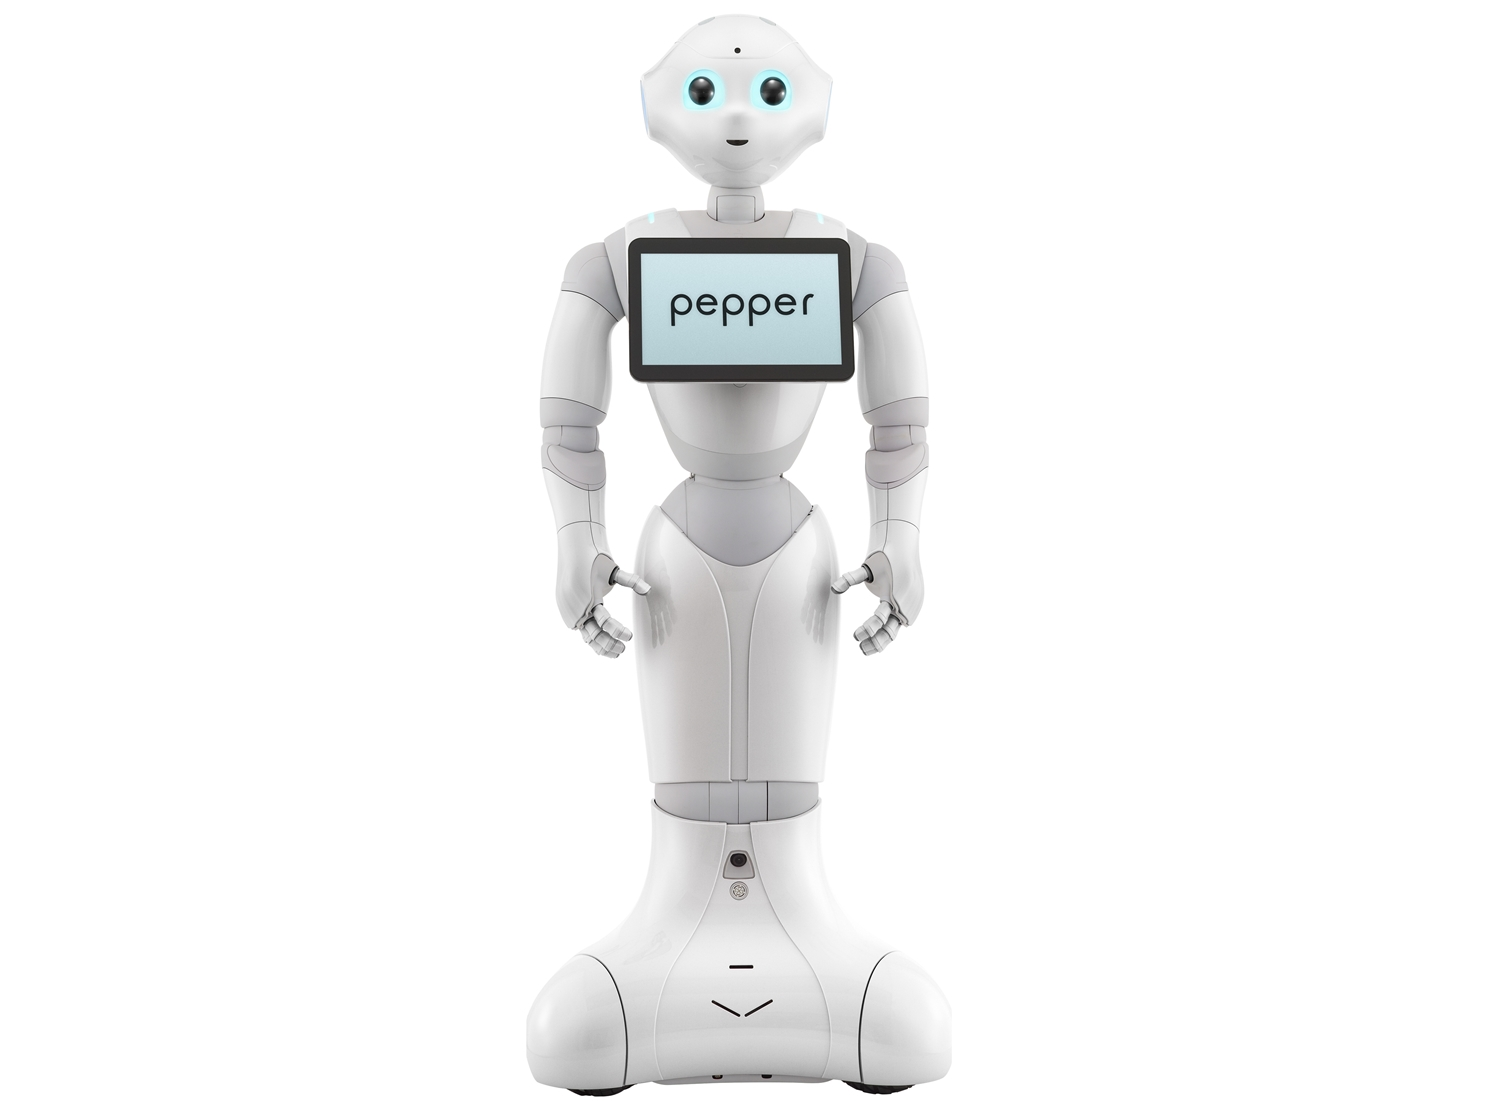
\includegraphics[height=7cm]{images/pepper.jpg}
	\caption{Le robot humanoïde Pepper.}
	\label{fig:Robot humanoïde Pepper}
\end{figure}

\paragraph{Caractéristiques techniques}
Caractéristiques techniques de la dernière version commerciale de Pepper (V1.5). \ref{tab: Caractéristiques technique de Pepper}

\begin{table}[h]
\begin{tabular}{ | l | p{8cm} | }
	\hline
	\multicolumn{2}{|c|}{Caractéristiques générales} \\
	\hline
	Dimensions & 1210 x 480 x 425 mm \\
	\hline 
	masse & 28 kg \\
	\hline 
	Degrés de liberté  & 17 \\
	\hline
	Processeur & Intel Atom E3845 \newline 1.91 GHz \newline RAM: 4 GB \newline Mémoire flash: 8 GB \newline MICRO SDHC: 16Go  \\
	\hline
	Système d'exploitation & Middleware Aldebaran NAOqi,\newline basé sur un noyau Linux \\
	\hline
	Connectivité & Wi-Fi, Ethernet, USB \\
	\hline
	Batterie & Énergie: 795 Wh \\
	\hline 
	Vision & 2 caméras 2D \newline 1 caméra 3D \\
	\hline
	Audio & 3 microphones directionnels \newline moteur de reconnaissance vocale Nuance  \\
	\hline
	Connectivité & Wi-Fi, Ethernet \\
	\hline
	Capteurs & 6 lasers, 2 capteurs infra-rouges, 1 système sonar, résistance sensible à la pression, 2 centrales inertielles, 3 surfaces tactiles \\
	\hline
\end{tabular}
\caption[Caractéristiques technique de Pepper]{Caractéristiques techniques de la dernière version commerciale  de Pepper}
\label {tab: Caractéristiques technique de Pepper}
\cite{PepperTech}
\end{table}

\subsection{Roméo}
\label{Entreprise: Les produits: Roméo}
Roméo est un nouveau type de robot d'accompagnement et d'assistance à la personne. Cette plateforme de recherche est soutenue par Aldebaran ainsi que d'autres partenaires universitaires et laboratoires de recherche (e.g. INRIA, LAAS-CNRS, ISIR, ENSTA, Telecom, etc.). Roméo est actuellement au stade de prototype et sert principalement de plateforme de tests pour les prochaines innovations majeures d'Aldebaran (e.g. les yeux mobiles, le système vestibulaire, etc.). 

\begin{figure}[h]
	\centering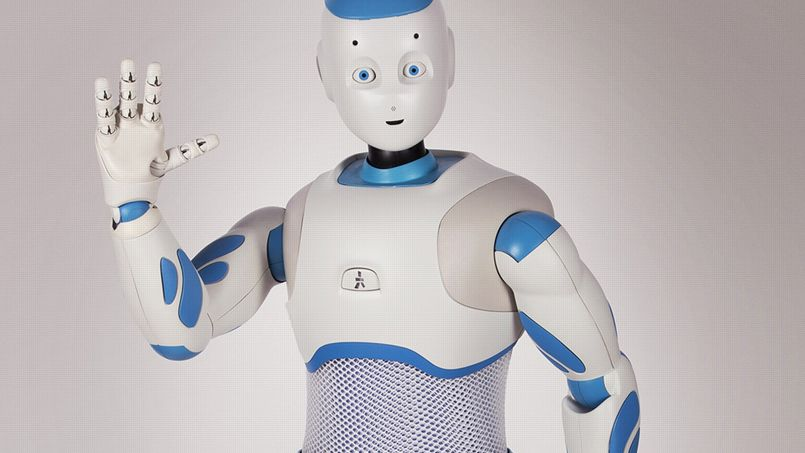
\includegraphics[height=6cm]{images/romeo.jpg}
	\caption{Le robot humanoïde Roméo.}
	\label{fig:Robot humanoïde Roméo}
\end{figure}

\paragraph{Caractéristiques techniques}
Caractéristiques techniques de la dernière version commerciale de Roméo (V2). \ref{tab: Caractéristiques technique de Roméo}

\begin{table}[h]
	\begin{tabular}{ | l | p{8cm} | }
		\hline
		\multicolumn{2}{|c|}{Caractéristiques générales} \\
		\hline
		Hauteur & 1467 mm \\
		\hline 
		masse & 37 kg \\
		\hline
		Processeur & Intel ATOM Z530 \newline 1.6 GHz \newline RAM: 1 GB \newline Mémoire flash: 2 GB \newline MICRO SDHC: 8 Go  \\
		\hline
		Système d'exploitation & Middleware Aldebaran NAOqi,\newline basé sur un noyau Linux \\
		\hline
		Connectivité & Wi-Fi, Ethernet \\
		\hline
		Batterie & Énergie: 795 Wh \\
		\hline 
		Vision & 4 caméras 2D \newline 1 caméra 3D \\
		\hline
		Audio & 3 microphones directionnels \newline moteur de reconnaissance vocale Nuance  \\
		\hline
		Connectivité & Wi-Fi, Ethernet \\
		\hline
		Capteurs & 6 lasers, 2 capteurs infra-rouges, 1 système sonar, résistance sensible à la pression, 2 centrales inertielles, 3 surfaces tactiles \\
		\hline
	\end{tabular}
	\caption[Caractéristiques technique de Roméo]{Caractéristiques techniques de la dernière version de Roméo}
	\label {tab: Caractéristiques technique de Roméo}
	\cite{RomeoTech}
\end{table}

\subsection{Le système d'exploitation NAOqi}
\label{Entreprise: Les produits: NAOqi}
NAOqi est le système d'exploitation commun aux robots d'Aldebaran. Il se base sur la distribution de Linux Gentoo et contient plusieurs API's afin de commander et contrôler les robots \cite{NAOqiTech}.
\begin{description}
	\item [NAOqi Core:] Gestion de l'ensemble des fonctions de base des robots (e.g. mémoire, "autonomous Life", comportements du robots, etc.).
	\item [NAOqi Motion:] Gestion des mouvements des robots.
	\item [NAOqi Audio:]  Gestion de la partie audio des robots.
	\item [NAOqi Vision:] Gestion de la partie vidéo des robots
	\item [NAOqi People Perception:] Ce module est utilisé pour étudier les personnes présentes autour du robot.
	\item [NAOqi Sensors:]  Gestion de l'ensemble des senseurs équipant les robots.
\end{description} 


\subsection{Plateforme de développement}
\label{Entreprise:Les produits: Nao: Plateforme de développement}
Les robots sont fournis avec une plateforme de développement.
\begin{description}
	\item[Choregraphe:] Il s'agit d'un outil de programmation graphique basé sur une interface prenant la forme de schémas bloc. Il permet de façon simple d'interagir avec le robot et de concevoir des applications pour le robot. Il comporte également un environnement de simulation 3D permettant aux développeurs de tester leurs applications sans même posséder un robot. Le logiciel permet également de disposer d'un retour visuel sur ce que le robot perçoit (e.g. vidéo issues des caméras, données des moteurs, etc.)
	
	\item[Kit de développement (SDK):] Il permet de développer des applications pour les robots via plusieurs langages de programmation:  C++, Python et Java.
\end{description}

